%%%%%%%%%%%%%%%%%%%%%%%%%%%%%%%%%%%%%%%%%
% Beamer Presentation
% LaTeX Template
% Version 1.0 (10/11/12)
%
% This template has been downloaded from:
% http://www.LaTeXTemplates.com
%
% License:
% CC BY-NC-SA 3.0 (http://creativecommons.org/licenses/by-nc-sa/3.0/)
%
%%%%%%%%%%%%%%%%%%%%%%%%%%%%%%%%%%%%%%%%%

%----------------------------------------------------------------------------------------
%	PACKAGES AND THEMES
%----------------------------------------------------------------------------------------

\documentclass{beamer}

\mode<presentation> {

% The Beamer class comes with a number of default slide themes
% which change the colors and layouts of slides. Below this is a list
% of all the themes, uncomment each in turn to see what they look like.

%\usetheme{default}
%\usetheme{AnnArbor}
%\usetheme{Antibes}
%\usetheme{Bergen}
%\usetheme{Berkeley}
%\usetheme{Berlin}
%\usetheme{Boadilla}
%\usetheme{CambridgeUS}
%\usetheme{Copenhagen}
%\usetheme{Darmstadt}
%\usetheme{Dresden}
%\usetheme{Frankfurt}
%\usetheme{Goettingen}
%\usetheme{Hannover}
%\usetheme{Ilmenau}
%\usetheme{JuanLesPins}
%\usetheme{Luebeck}
%\usetheme{Madrid}
%\usetheme{Malmoe}
%\usetheme{Marburg}
%\usetheme{Montpellier}
%\usetheme{PaloAlto}
%\usetheme{Pittsburgh}
%\usetheme{Rochester}
%\usetheme{Singapore}
%\usetheme{Szeged}
%\usetheme{Warsaw}
\usetheme{Amsterdam}

% As well as themes, the Beamer class has a number of color themes
% for any slide theme. Uncomment each of these in turn to see how it
% changes the colors of your current slide theme.

%\usecolortheme{albatross}
%\usecolortheme{beaver}
%\usecolortheme{beetle}
%\usecolortheme{crane}
%\usecolortheme{dolphin}
%\usecolortheme{dove}
%\usecolortheme{fly}
%\usecolortheme{lily}
%\usecolortheme{orchid}
%\usecolortheme{rose}
%\usecolortheme{seagull}
%\usecolortheme{seahorse}
%\usecolortheme{whale}
%\usecolortheme{wolverine}

%\setbeamertemplate{footline} % To remove the footer line in all slides uncomment this line
%\setbeamertemplate{footline}[page number] % To replace the footer line in all slides with a simple slide count uncomment this line

%\setbeamertemplate{navigation symbols}{} % To remove the navigation symbols from the bottom of all slides uncomment this line
}

\usepackage{graphicx} % Allows including images
\usepackage{booktabs} % Allows the use of \toprule, \midrule and \bottomrule in tables
\usepackage[utf8]{inputenc}
% http://tex.stackexchange.com/questions/107637/repeated-division-converting-from-base-10-to-another-base


\newcount\total
\newcount\lasttotal
\newcount\targetbase

\def\digittoalpha#1{%
    \ifcase#1\relax0\or1\or2\or3\or4\or5\or6\or7\or8\or9%
    \or a\or b\or c\or d\or e\or f\or g\or h\or i\or j\or k\or l\or m%
    \or n\or p\or p\or q\or r\or s\or t\or u\or v\or w\or x\or y\or z\else?\fi%
}

\def\baseconversiontable#1#2{%
    \begin{tikzpicture}[every node/.style={minimum width=1cm, minimum height=0.5cm}, x=1cm,y=0.5cm]
    %
    \total=#1%
    \targetbase=#2
    \def\newnumber{}
    %
    \pgfmathloop
    \ifnum\total<1
    \else
        %
        \ifnum\pgfmathcounter>1
            \node at (\pgfmathcounter, -\pgfmathcounter+1) (tmp) {\the\targetbase};
            \draw (tmp.north west) |- (tmp.south east);
            %
            \node at (\pgfmathcounter-1, -\pgfmathcounter) (tmp) {\pgfmathparse{int(-\total*\targetbase)}\pgfmathresult};
            \draw (tmp.south west) -- (tmp.south east);
            %
            \pgfmathparse{int(\lasttotal-\total*\targetbase)}%
            \let\digit=\pgfmathresult
            \node at (\pgfmathcounter-1, -\pgfmathcounter-1) [text=red] {\digit};
            \edef\newnumber{\digit\newnumber}
        \fi
        %
        \ifnum\total<\targetbase
            \edef\currentdigit{\uppercase{\digittoalpha{\the\total}}}%
            \edef\newnumber{\currentdigit\newnumber}
            \ifnum\total>9
              \edef\currentdigit{\noexpand\rm{\currentdigit}}%
            \fi
            \node at (\pgfmathcounter, -\pgfmathcounter) [text=red]  {\the\total};
            %\color{black}\the\total(\color{red}\currentdigit\color{black})
            %};
        \else
            \node at (\pgfmathcounter, -\pgfmathcounter) {\the\total};
        \fi
        \lasttotal=\total
        \divide\total by\targetbase
    \repeatpgfmathloop    
    \draw [->] (\pgfmathcounter-1,-\pgfmathcounter-1) -- ++(-0.5,0); 
    %\node [anchor=west] at (1, -\pgfmathcounter-2) {$#1=\newnumber_{\the\targetbase}$};
    \end{tikzpicture}   
}



\usepackage{framed}

\usepackage{algorithm}
\usepackage[noend]{algpseudocode}
\definecolor{algocoul}{rgb}{0,0,0.75}
\definecolor{algocom}{rgb}{.75,.25,0}
\floatname{algorithm}{Algorithme}

\usepackage{tikz}
\usepackage{tikz-timing}
\usepackage{tkz-graph} 
\usetikzlibrary{arrows,shapes.gates.logic.US,shapes.gates.logic.IEC,calc,shapes.geometric,positioning}
\tikzset{
  multiplexer/.style={
    draw,
    trapezium,
    shape border uses incircle, 
    shape border rotate=270,
    minimum size=18pt
  }  
}

\tikzset{
    alu/.style={trapezium,
            trapezium angle=26,
            shape border rotate=180,
            minimum width=3cm,
            minimum height=2cm,
            trapezium stretches=true,
            append after command={%
                    \pgfextra
                        \draw (\tikzlastnode.top left corner) --
                           (\tikzlastnode.top right corner) -- 
                           (\tikzlastnode.bottom right corner) -- 
                           ($(\tikzlastnode.bottom right corner)!.666!(\tikzlastnode.bottom side)$)--
                           ([yshift=-1cm]\tikzlastnode.bottom side)--
                           ($(\tikzlastnode.bottom side)!.334!(\tikzlastnode.bottom left corner)$)--
                           (\tikzlastnode.bottom left corner)--
                           (\tikzlastnode.top left corner);
                    \endpgfextra}},
}




\usepackage[europeanresistors, siunitx]{circuitikz}

\usepackage{listings}

%----------------------------------------------------------------------------------------
%	TITLE PAGE
%----------------------------------------------------------------------------------------

\title[Architecture]{Architecture des ordinateurs} % The short title appears at the bottom of every slide, the full title is only on the title page

\author{Jérémy Fix} % Your name
\institute[CS] % Your institution as it will appear on the bottom of every slide, may be shorthand to save space
{
CentraleSupélec \\ % Your institution for the title page
\medskip
\textit{jeremy.fix@centralesupelec.fr} % Your email address
}
\date{2017-2018} % Date, can be changed to a custom date

\begin{document}

\begin{frame}
\titlepage % Print the title page as the first slide
\end{frame}

%% \begin{frame}
%% \frametitle{Overview} % Table of contents slide, comment this block out to remove it
%% \tableofcontents % Throughout your presentation, if you choose to use \section{} and \subsection{} commands, these will automatically be printed on this slide as an overview of your presentation
%% \end{frame}

%----------------------------------------------------------------------------------------
%	PRESENTATION SLIDES
%----------------------------------------------------------------------------------------



\section{Petite synthèse}

\begin{frame}
\begin{center}
\frametitle{Petit retour sur l'architecture v0}
\centering\includegraphics[width=\linewidth]{Figs/premier_chemin_seq_jmp.pdf}
\end{center}
\end{frame}

\begin{frame}
\frametitle{Architecture à Jeu d'instructions (ISA)}
\begin{tiny}
\begin{tabular}{cccp{10cm}}
Code instruction & Nom & Mots & Description \\
\hline
0x0c00 & END & 1 & Fin du programme\\
0x1000 & LDAi & 2 & Charge la valeur de l'opérande dans le registre A. [A:=opérande]\\
0x1400 & LDAd & 2 & Charge la valeur dans la RAM pointée par l'opérande dans le registre A. [A:=Mem[opérande]].\\
0x1c00 & STA & 2 & Sauvegarde en mémoire la valeur du registre A à l'adresse donnée par l'opérande. [Mem[opérande]:= A]\\
0x2000 & LDBi & 2 & Charge la valeur de l'opérande dans le registre B. [B:=opérande]\\
0x2400 & LDBd & 2 & Charge la valeur dans la RAM pointée par l'opérande dans le registre B. [B:=Mem[opérande]].\\
0x2c00 & STB & 2 & Sauvegarde en mémoire la valeur du registre B à l'adresse donnée par l'opérande. [Mem[opérande]:= B]\\
0x3000 & ADDA &	1 &Ajoute le contenu des registres A et B et mémorise le résultat dans le registre A. [A:=A+B]\\
0x3400 & ADDB &1 &Ajoute le contenu des registres A et B et mémorise le résultat dans le registre B. [B:=A+B]\\
0x3800 & SUBA & 1 &Soutstrait le contenu des registres A et B et mémorise le résultat dans le registre A. [A:=A-B]\\
0x3c00&	SUBB &1 &Soutstrait le contenu des registres A et B et mémorise le résultat dans le registre B. [B:=A-B]\\
0x4000& MULA &1 &Multiplie le contenu des registres A et B et mémorise le résultat dans le registre A. [A:=AxB] \\
0x4400&	MULB &1 &Multiplie le contenu des registres A et B et mémorise le résultat dans le registre B. [B:=AxB]\\
0x4800& DIVA &1 &Divise le contenu du registre A par deux et mémorise le résultat dans A. [A:=A/2]\\
0x5000&	ANDA &1 & Calcule un ET logique entre le contenu des registres A et B et mémorise le résultat dans A. [A:=A\&B]\\
0x5400&	ANDB &1 & Calcule un ET logique entre le contenu des registres A et B et mémorise le résultat dans B. [B:=A\&B]\\
0x5800&	ORA  &1 & Calcule un OU logique entre le contenu des registres A et B et mémorise le résultat dans A. [A:=A|B]\\
0x5c00&	ORB  &1 & Calcule un OU logique entre le contenu des registres A et B et mémorise le résultat dans B. [B:=A|B]\\
0x6000&	NOTA &1 & Mémorise dans A la négation de A. [A:=!A]\\
0x6400&	NOTB &1 &Mémorise dans B la négation de B. [B:=!B]\\
0x7000&	JMP  &2 &Saute inconditionnellement à l'adresse donnée par l'opérande. [PC:=operande]\\
0x7400&	JZA  &2 &Saute à l'adresse donnée par l'opérande si le contenu du registre A est nul. [PC:=operande si A=0]\\
0x7800&	JZB  &2 &Saute à l'adresse donnée par l'opérande si le contenu du registre B est nul. [PC := operande si B=0]
\end{tabular}
\end{tiny}

\end{frame}

\begin{frame}
\frametitle{Automate à états finis du séquenceur}

  \centering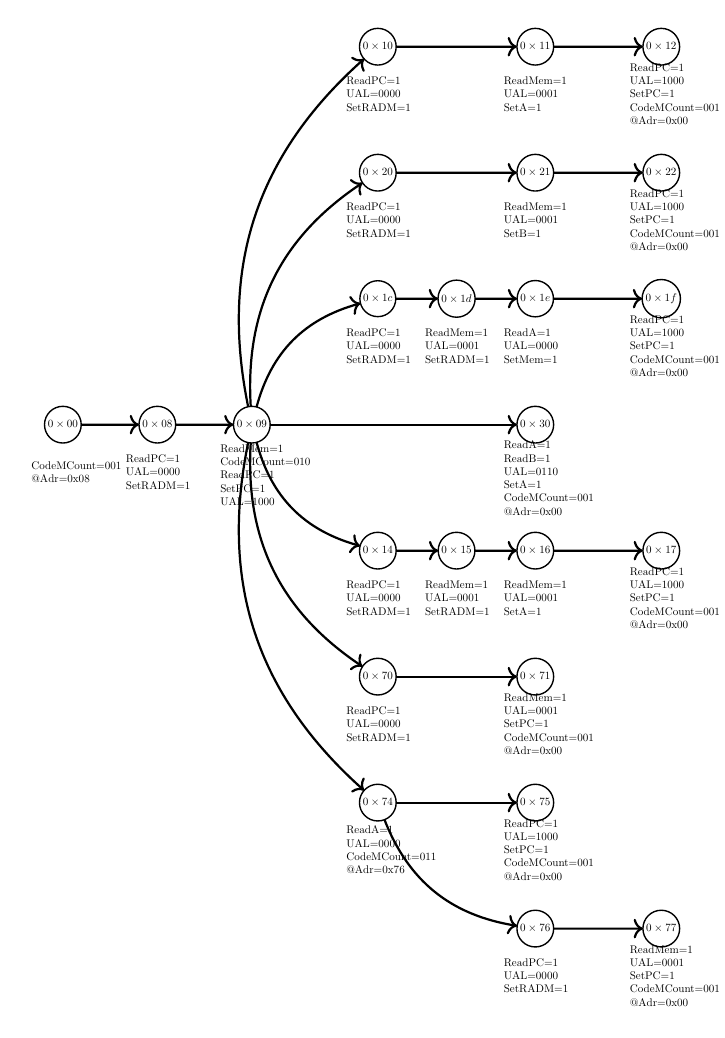
\begin{tikzpicture}[thick,scale=0.4, every node/.style={scale=0.4}]
    GraphInit[vstyle=Normal]
    \SetGraphUnit{3}
    \tikzset{LabelStyle/.style= {draw,
        fill  = white,
        text  = blue},
      EdgeStyle/.style = {->}}
    \Vertex[Math,L=0\times00,x=-10,y=8]{A0}
    \Vertex[Math,L=0\times08,x=-7,y=8]{B0}
    \Vertex[Math,L=0\times09,x=-4,y=8]{C0}
    \Edge(A0)(B0)
    \Edge(B0)(C0)
    \node[text width=2cm] at ($(A0) - (0,1.5)$) {CodeMCount=001\\ @Adr=0x08} ;
    \node[text width=2cm] at ($(B0) - (0,1.5)$) {ReadPC=1\\UAL=0000\\SetRADM=1} ;
    \node[text width=2cm] at ($(C0) - (0,1.6)$) {ReadMem=1\\CodeMCount=010\\ ReadPC=1\\SetPC=1\\UAL=1000} ;


    \Vertex[Math,L=0\times10,x=0,y=20]{A1}
    \Vertex[Math,L=0\times11,x=5,y=20]{B1}
    \Vertex[Math,L=0\times12,x=9,y=20]{C1}
    \Edge(A1)(B1)
    \Edge(B1)(C1)
    \node[text width=2cm] at ($(A1) - (0,1.5)$) {ReadPC=1\\UAL=0000\\SetRADM=1} ;
    \node[text width=2cm] at ($(B1) - (0,1.5)$) {ReadMem=1\\UAL=0001\\SetA=1} ;
    \node[text width=2cm] at ($(C1) - (0,1.5)$) {ReadPC=1\\UAL=1000\\SetPC=1\\CodeMCount=001\\@Adr=0x00} ;

    \Vertex[Math,L=0\times20,x=0,y=16]{A2}
    \Vertex[Math,L=0\times21,x=5,y=16]{B2}
    \Vertex[Math,L=0\times22,x=9,y=16]{C2}
    \Edge(A2)(B2)
    \Edge(B2)(C2)
    \node[text width=2cm] at ($(A2) - (0,1.5)$) {ReadPC=1\\UAL=0000\\SetRADM=1} ;
    \node[text width=2cm] at ($(B2) - (0,1.5)$) {ReadMem=1\\UAL=0001\\SetB=1} ;
    \node[text width=2cm] at ($(C2) - (0,1.5)$) {ReadPC=1\\UAL=1000\\SetPC=1\\CodeMCount=001\\@Adr=0x00} ;


    \Vertex[Math,L=0\times1c,x=0,y=12]{A3}
    \Vertex[Math,L=0\times1d,x=2.5,y=12]{B3}
    \Vertex[Math,L=0\times1e,x=5,y=12]{C3}
    \Vertex[Math,L=0\times1f,x=9,y=12]{D3}
    \Edge(A3)(B3)
    \Edge(B3)(C3)
    \Edge(C3)(D3)
    \node[text width=2cm] at ($(A3) - (0,1.5)$) {ReadPC=1\\UAL=0000\\SetRADM=1} ;
    \node[text width=2cm] at ($(B3) - (0,1.5)$) {ReadMem=1\\UAL=0001\\SetRADM=1} ;
    \node[text width=2cm] at ($(C3) - (0,1.5)$) {ReadA=1\\UAL=0000\\SetMem=1} ;
    \node[text width=2cm] at ($(D3) - (0,1.5)$) {ReadPC=1\\UAL=1000\\SetPC=1\\CodeMCount=001\\@Adr=0x00} ;


    \Vertex[Math,L=0\times30,x=5,y=8]{A4}
    \node[text width=2cm] at ($(A4) - (0,1.7)$) {ReadA=1\\ReadB=1\\UAL=0110\\SetA=1\\CodeMCount=001\\@Adr=0x00} ;

    \Vertex[Math,L=0\times14,x=0,y=4]{A5}
    \Vertex[Math,L=0\times15,x=2.5,y=4]{B5}
    \Vertex[Math,L=0\times16,x=5,y=4]{C5}
    \Vertex[Math,L=0\times17,x=9,y=4]{D5}
    \Edge(A5)(B5)
    \Edge(B5)(C5)
    \Edge(C5)(D5)
    \node[text width=2cm] at ($(A5) - (0,1.5)$) {ReadPC=1\\UAL=0000\\SetRADM=1} ;
    \node[text width=2cm] at ($(B5) - (0,1.5)$) {ReadMem=1\\UAL=0001\\SetRADM=1} ;
    \node[text width=2cm] at ($(C5) - (0,1.5)$) {ReadMem=1\\UAL=0001\\SetA=1} ;
    \node[text width=2cm] at ($(D5) - (0,1.5)$) {ReadPC=1\\UAL=1000\\SetPC=1\\CodeMCount=001\\@Adr=0x00} ;


    \Vertex[Math,L=0\times70,x=0,y=0]{A6}
    \Vertex[Math,L=0\times71,x=5,y=0]{B6}
    \Edge(A6)(B6)
    \node[text width=2cm] at ($(A6) - (0,1.5)$) {ReadPC=1\\UAL=0000\\SetRADM=1} ;
    \node[text width=2cm] at ($(B6) - (0,1.5)$) {ReadMem=1\\UAL=0001\\SetPC=1\\CodeMCount=001\\@Adr=0x00} ;

    \Vertex[Math,L=0\times74,x=0,y=-4]{A7}
    \Vertex[Math,L=0\times75,x=5,y=-4]{B7}
    \Vertex[Math,L=0\times76,x=5,y=-8]{C7}
    \Vertex[Math,L=0\times77,x=9,y=-8]{D7}
    \Edge(A7)(B7)
    \Edge[style={->,bend right}](A7)(C7)
    \Edge(C7)(D7)
    \node[text width=2cm] at ($(A7) - (0,1.5)$) {ReadA=1\\UAL=0000\\CodeMCount=011\\ @Adr=0x76} ;
    \node[text width=2cm] at ($(B7) - (0,1.5)$) {ReadPC=1\\UAL=1000\\SetPC=1\\CodeMCount=001\\@Adr=0x00} ;
    \node[text width=2cm] at ($(C7) - (0,1.5)$) {ReadPC=1\\UAL=0000\\SetRADM=1} ;
    \node[text width=2cm] at ($(D7) - (0,1.5)$) {ReadMem=1\\UAL=0001\\SetPC=1\\CodeMCount=001\\ @Adr=0x00} ;



    \Edge[style={->,bend left}](C0)(A1)
    \Edge[style={->,bend left}](C0)(A2)
    \Edge[style={->,bend left}](C0)(A3)
    \Edge[style={->}](C0)(A4)
    \Edge[style={->,bend right}](C0)(A5)
    \Edge[style={->,bend right}](C0)(A6)
    \Edge[style={->,bend right}](C0)(A7)
  \end{tikzpicture}

\end{frame}

\begin{frame}
\frametitle{Séquenceur et programme}

\begin{block}{Séquenceur}
\begin{itemize}
\item Sémantique des instructions
\item Générique
\item Automate à états finis : état dans MicroPC, signaux de contrôle ROM[MicroPC]
\end{itemize}
\end{block}

\begin{block}{Programme}
\begin{itemize}
\item Qu'est ce que je veux calculer ?
\item Spécifique 
\item Séquence de codes d'instructions et de données en RAM
\end{itemize}
\end{block}
\end{frame}

\begin{frame}
  \frametitle{Aperçu de quelques architectures}
  \begin{block}{La notre}
    \begin{itemize}
    \item 2 registres banalisés : A et B
    \item 2 registres internes : RADM et PC
    \item adresses sur 16 bits, données sur 16 bits
    \item 1 mot de 16 bit pour l'instruction, 1 mot pour l'opérande éventuelle
    \item jeu d'instructions : LDAi, LDBi, ADDA, ANDB, JMP, JZA
    \item horloge maximale sous logisim : 4 kHz
    \end{itemize}
  \end{block}
  Beaucoup d'architectures :\\\url{https://en.wikipedia.org/wiki/List_of_instruction_sets}
\end{frame}

%%% https://www.cs.umd.edu/users/meesh/webpages/cmsc311/links/handouts/huang-ia32.pdf
\begin{frame}
  \frametitle{Aperçu de quelques architectures}
  \begin{block}{Intel x86 IA32-64}
    Du Intel 8086(1978) jusqu'au Intel Core i7 (2015)
    \begin{itemize}
    \item 8 registres banalisés 32 bits EAX, EBX, ECX, EDX, ESI, EDI, EBP, ESP
    \item 6 registres de segments 16 bits : CS, DS, SS,ES, FS, GS
    \item 1 registre de status 32 bits : EFLAGS
    \item x registres internes : EIP (32 bits)
    \end{itemize}
  \end{block}
  \begin{small}
  Intel 64 and IA-32 Architectures Software Developer Manuals \url{https://software.intel.com/en-us/articles/intel-sdm}\end{small}
\end{frame}

\begin{frame}
  \frametitle{Aperçu de quelques architectures}
  \begin{block}{Intel x86 IA32-64}
    Le registre de statut EFLAGS\\
    \begin{center}
      \includegraphics[width=0.7\columnwidth]{Figs/x86_eflags.png}
    \end{center}    
  \end{block}
\end{frame}
  
%% Comment faire pour charger une valeur immédiate de 32 bits ??
%% https://www.cs.umd.edu/class/sum2003/cmsc311/Notes/Mips/load32.html
%% dans une instruction qui ne fait que 32 bits ....

%% Instructions : http://flint.cs.yale.edu/cs422/doc/24547112.pdf#page=60&zoom=auto,-213,719
\begin{frame}
  \frametitle{Aperçu de quelques architectures}
  \begin{block}{Intel x86 IA32-64: Jeu d'instructions}
    Beaucoup d'instructions : 1.300 mnémoniques, plusieurs modes d'adressages, ..\\
    \begin{center}
      \includegraphics[width=0.6\columnwidth]{Figs/ia32_instructions.png}
    \end{center}
    Opérations arithmétiques : ADD(0x01, 0x02, 0x03), AND(0x21,0x22, ..)..\\
    Branchements (in)conditionnels: JMP (0xFF), JZ, JNZ, JG, conditions à partir des bits de statut\\
    Lecture/Ecriture : MOV(0x8B, 0xC7, ...)
  \end{block}
\end{frame}

\begin{frame}
  \frametitle{Aperçu de quelques architectures}
  \begin{block}{ARM (téléphones, tablettes, consoles)}
    Acorn RISC Machine architecture (1980) jusqu'au ARMv8.3-A (2016)
    \begin{itemize}
    \item 16 registres $Ri$ 32 bits dont~:
      \begin{itemize}
      \item $R0-R3$ : arguments/résultats pour une routine
      \item $R4-R8$ : variables temporaires
      \item $R9$ : Plateform register
      \item $R10$ : Stack limit pointer
      \item $R11$ : Frame pointer
      \item $R12$ : registre temporaire
      \item $R13$ : Stack Pointer
      \item $R14$ : Link register (adresse de retour)
      \item $R15$ : Programm Counter
      \end{itemize}
    \item 1 registre de statut CPSR 32 bits
    \end{itemize}
  \end{block}
  \url{http://infocenter.arm.com/help/index.jsp}
\end{frame}


\begin{frame}
  \frametitle{Aperçu de quelques architectures}
  \begin{block}{ARM (téléphones, tablettes, consoles)}
    Le registre CPSR\\
    \includegraphics[width=\columnwidth]{Figs/arm_cpsr.png}
  \end{block}
\end{frame}
  
\begin{frame}
  \frametitle{Aperçu de quelques architectures}
  \begin{block}{ARM - Jeu d'instructions}
    Data Processing avec opcode: AND(0000), ADD(0100), SUB(0010)\\
    \includegraphics[width=0.8\columnwidth]{Figs/arm_dataprocessing.png}\\
    Branchements~: BX, BL, ..\\
    \includegraphics[width=0.8\columnwidth]{Figs/arm_branch.png}\\
    et bien d'autres...
  \end{block}
  \url{http://infocenter.arm.com/help/index.jsp}
\end{frame}


\begin{frame}
\frametitle{La v0 est conçue, programmons la !}

\begin{block}{Conception}
\begin{minipage}[l]{0.45\linewidth}
\begin{itemize}
\item Chemin de données
\item Jeu d'instructions
\item Séquenceur
\end{itemize}
\end{minipage}
\begin{minipage}[c]{0.5\linewidth}
  \includegraphics[width=\columnwidth]{Figs/lego-builder.jpg}
\end{minipage}
\end{block}
\begin{block}{Programmation}
\begin{minipage}[l]{0.45\linewidth}
\begin{itemize}
\item Code machine (instructions/données)
\item Calcul des adresses ``à la main''
\begin{itemize}
\item adresses des branchements?
\item adresses des données ?
\end{itemize}
\end{itemize}
\end{minipage}
\begin{minipage}[c]{0.5\linewidth}
  \includegraphics[width=\columnwidth]{Figs/lego-programmer.jpg}
\end{minipage}
\end{block}

\end{frame}


\begin{frame}
\frametitle{C'est dur et long pour le moment de programmer}

\begin{block}{Calculer la suite de Syracuse}
\begin{align*}
\forall n \in \mathbb{N}^*, u_{n+1} &=
\begin{cases}
u_n/2 & \mbox{si } u_n \mbox{ est pair}\\
3u_{n+1}+1 & \mbox{ sinon}
\end{cases}\\
u_0 &= 127 ; u_{n} = ?
\end{align*}
\end{block}
$\Leftrightarrow$
\begin{block}{Code machine}
1000 007f 1c00 0024  1c00 1000 1400 0024 2000 0001 5000 7400 001b
1400 0024 2000 0003 4000 2000 0001 3000 1c00 0024 1c00 1000 7000 0006 
1400 0024 4800 1c00 0024 1c00 1000 7000 0006 
\end{block}
si si, je vous assure. Donc, c'est dur et long.
\end{frame}

\begin{frame}
\frametitle{C'est dur et long pour le moment de programmer}

\begin{block}{Calculer la suite de Syracuse}
\begin{align*}
\forall n \in \mathbb{N}^*, u_{n+1} &=
\begin{cases}
u_n/2 & \mbox{si } u_n \mbox{ est pair}\\
3u_{n+1}+1 & \mbox{ sinon}
\end{cases}\\
u_0 &= 127 ; u_{n} = ?
\end{align*}
\end{block}
$\Leftrightarrow$
\begin{block}{Code machine}
[LDAi 007f STA 0024  STA 1000] [LDAd 0024 LDBi 0001 ANDA JZA \textbf{001b}]
[LDAd 0024 LDBi 0003 MULA LDBi 0001 ADDA STA 0024 STA 1000 JMP \textbf{0006}] 
[LDAd 0024 DIVA STA 0024 STA 1000 JMP \textbf{0006}]
\end{block}
\end{frame}


\begin{frame}
\frametitle{Comment faire pour simplifier la programmation ?}

\begin{block}{Ne plus écrire en code machine\footnote{parfois utile tout de même}}
\begin{footnotesize}
\begin{tabular}{ccccc}
Code machine (arg..) & & Assemblage (cool!) & & Python (super cool!)\\
\begin{tabular}{l}
1000 0001\\
 2000 0002\\
 3000 
\end{tabular}& $\xleftarrow{\mathtt{???}}$ & 
\begin{tabular}{l}
LDAi 1\\
LDBi 2\\
ADDA\end{tabular}
& $\xleftarrow{\mathtt{???}}$ & 
\begin{tabular}{l}
a=1\\ b=2\\ a=a+b
\end{tabular}
\end{tabular}
\end{footnotesize}
\end{block}
\begin{itemize}
\item Langage d'assemblage ? LDAi, STA, ADDA, ..
\item Langages de haut-niveau (architecture indépendant) : C++, Python, .. ?
\end{itemize}
et bien sûr comment faire la conversion vers le langage machine
\end{frame}

\begin{frame}[fragile]
\frametitle{Comment faire pour simplifier la programmation ?}

\begin{block}{Les procédures (ou fonctions)}
Définition : succession d'opérations à exécuter pour accomplir une tâche déterminée [Larousse]
\end{block}

Exemple de Syracuse en Python: \\
\begin{minipage}[c]{0.45\textwidth}
Sans procédures
\begin{center}
\begin{footnotesize}
\begin{verbatim}
un = 127
if(un % 2 == 0):
   un = un/2
else:
   un = 3 un + 1
if(un % 2 == 0):
   un = un/2
else:
   un = 3 un + 1
if(un % 2 == 0):
   un = un/2
else:
   un = 3 un + 1
\end{verbatim}
\end{footnotesize}
\end{center}
\end{minipage}
\begin{minipage}[c]{0.45\textwidth}
Avec procédures
\begin{center}
\begin{footnotesize}
\begin{verbatim}
def f(u):
    if(u % 2 == 0):
       return u/2
    else:
       return 3 * u + 1

u = 127
u = f(u)
u = f(u)
\end{verbatim}
\end{footnotesize}
\end{center}
\vfill
\end{minipage}


\end{frame}


\begin{frame}
\frametitle{On a presque des procédures}

\begin{block}{Syrarcuse}
\centering\includegraphics[width=0.7\linewidth]{Figs/call_pc.pdf}
\end{block}
\begin{block}{}
\begin{itemize}
\item programme de $f$ : $0\times 0014$
\item on utilise ici explicitement le registre A pour stocker les arguments et le résultat
\item retour ?
\end{itemize}
\end{block}

\end{frame}

\begin{frame}
Nous avons donc trois problèmes à résoudre :
\begin{itemize}
\item comment partir exécuter la routine ? JMP
\item comment passer les arguments à la routine ? 
\begin{itemize}
\item Registres dédiés : combien ?? (e.g. $R0-R3$ pour ARM)
  \item autre chose ?
\end{itemize}
\item comment revenir au programme appelant ? 
\begin{itemize}
\item sauvegarder l'adresse de retour dans un registre dédié : \emph{link register} à sauvegarder lors d'appels cascadés  (A appelle B qui appelle C qui appelle ...), e.g. ARM
\item autre chose ?
\end{itemize}
\item comment récupérer le résultat ?
  \begin{itemize}
  \item un registre dédié ? (e.g. $R0$ pour ARM)
  \item autre chose ?
  \end{itemize}
\end{itemize}
\vspace{1cm}
Dans notre architecture, on va répondre à ces 3 questions en utilisant une structure particulière : \textbf{la pile}
\end{frame}

%------------------------------------------------
\section{Procédure, pile et pointeur de pile} 
%------------------------------------------------

\begin{frame}
\begin{center}
\textbf{Procédures, pile et pointeur de pile}\\
\vspace{1cm}
\centering\includegraphics[width=0.5\linewidth]{Figs/Lifo.png}
\end{center}
\end{frame}


\begin{frame}
\frametitle{Spécifications d'une pile}
\begin{block}{Une pile en mémoire}
\begin{itemize}
\item structure de données en mémoire principale (RAM)
\item empiler, dépiler une valeur : sommet de pile
\item ou est le sommet de pile : registre \emph{Stack Pointer}
\end{itemize}
\end{block}

\centering\includegraphics[width=0.5\linewidth]{Figs/Lifo.png}

\end{frame}

\begin{frame}
\frametitle{Ajout de SP dans le chemin de données}

\centering\includegraphics[width=\linewidth]{Figs/premier_chemin_seq_sp.pdf}

\end{frame}

\begin{frame}
\frametitle{Ajout d'instructions de manipulation de la pile}

\begin{block}{Spécifications}
\begin{itemize}
\item ou placer la pile en mémoire ?
\item quelle est l'adresse du sommet de la pile en mémoire ?
\item comment empiler/dépiler, écrire/lire des éléments de la pile ?
\end{itemize}
\end{block}

\begin{block}{Instructions particulières}
\begin{itemize}
\item pour manipuler le registre SP : LDSPi, STSP, INCSP, DECSP
\item pour empiler/dépile : PUSH\{A,B\}, POP\{A, B\}
\item pour lire/écrire relativement à SP : POKE\{A,B\}, PEEK\{A,B\}
\end{itemize}
\end{block}
\end{frame}

\begin{frame}
\frametitle{PUSH, POP, POKE, PEEK, Hum?!}

\centering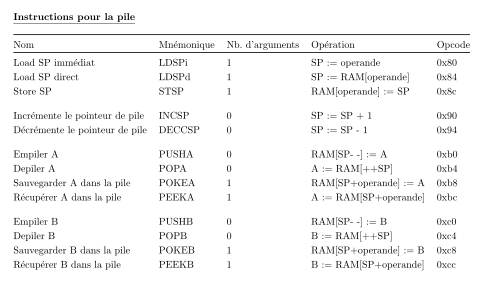
\includegraphics[width=\linewidth]{Figs/stack.pdf}\\

$\rightarrow$ Machines à états (b0, b4, b8, bc)?
\end{frame}

\begin{frame}
\frametitle{Utilisons la pile pour passer des arguments}

\begin{algorithmic}[1]
\Function{somme}{$N$}
\State{Soient $i$, $res$ deux variables locales}
\State{$i \gets N-1$}
\State{$res \gets 0$}
\While{$i \neq 0$}
\State{$res \gets res + i$}
\State{$i \gets i - 1$}
\EndWhile
\State \Return $res$
\EndFunction

\Function{main}{}
\State somme($3$)
\EndFunction
\end{algorithmic}

\end{frame}

\begin{frame}
\frametitle{Somme: Une première tentative}

\centering\includegraphics[width=\linewidth]{Figs/stack_args_noret.pdf}
\hrule
\centering\includegraphics[width=\linewidth]{Figs/stack_args_fig_no_ret.pdf}


\end{frame}

\begin{frame}
\frametitle{Appel et retour de routines}

\begin{block}{Spécifications}
\begin{itemize}
\item Quand on part exécuter le code d'une procédure, il faut sauvegarder là o{\`u} retourner (marque page)
\item Quand on termine une procédure, il faut poursuivre le programme appelant
\end{itemize}
\end{block}
\begin{block}{Instructions particulières}
\begin{itemize}
\item CALL (0xA000): ``\texttt{CALL op}'' Empile l'adresse de la \textbf{prochaine} instruction et branche
\item RET (0xA800): ``\texttt{RET}'' Dépile dans PC l'adresse de retour
\end{itemize}
\end{block}
\end{frame}


\begin{frame}
\frametitle{Réalisation de ces instructions}
\includegraphics[width=\linewidth]{Figs/stack_args_ret.pdf}
\end{frame}

\begin{frame}
\frametitle{Réalisation de ces instructions}
\includegraphics[width=\linewidth]{Figs/premier_chemin_seq_sp_tmp.pdf}
\end{frame}

\begin{frame}
\frametitle{Réalisation de ces instructions}
\includegraphics[width=\linewidth]{Figs/stack_args_ret.pdf}

et le résultat au fait? La pile !
\end{frame}


\begin{frame}
\frametitle{Somme : une deuxième tentative}

\centering\includegraphics[width=\linewidth]{Figs/stack_args_call.pdf}
\hrule
\centering\includegraphics[width=\linewidth]{Figs/stack_args_fig.pdf}

\end{frame}

\begin{frame}
\frametitle{Déroulement d'un appel de routine}

\begin{small}
Le programme appelant
\begin{itemize}
\item réserve de la place pour le résultat (DECSP)
\item empile les arguments (PUSH)
\item sauvegarde la valeur PC \underline{après lecture} de l'adresse de la routine et branche sur la routine (CALL)
\end{itemize}

Programme appelé
\begin{itemize}
\item lit les arguments dans la pile (PEEK), 
\item calcule son résultat éventuel et le sauvegarde dans la pile (POKE)
\item retourne au programme appelant (RET) : le registre SP doit être restauré!
\end{itemize}

Programme appelant
\begin{itemize}
\item dépile les arguments (INCSP ou POP)
\item dépile le résultat (POP) et se poursuit
\end{itemize}
\end{small}

\end{frame}

\begin{frame}
\frametitle{Qui met/enlève quoi dans la pile ?}

\centering\includegraphics[width=\linewidth]{Figs/respo_pile.pdf}

\begin{block}{Attention!}
Dans cette version d'architecture, les accès PEEK, POKE sont relatifs au sommet de pile !\\
Autre possibilité : registre Base Pointer (BP) / Frame Pointer (FP)\\
Pour restaurer le registre SP, on pourrait aussi utiliser BP/FP
\end{block}

\end{frame}

\begin{frame}
\frametitle{C'est parti pour le code machine de :}

\begin{algorithmic}[1]
\Function{somme}{$N$}
\State{Soient $i$, $res$ deux variables locales}
\State{$i \gets N-1$}
\State{$res \gets 0$}
\While{$i \neq 0$}
\State{$res \gets res + i$}
\State{$i \gets i - 1$}
\EndWhile
\State \Return $res$
\EndFunction

\Function{main}{}
\State somme($3$)
\EndFunction
\end{algorithmic}

\end{frame}


\begin{frame}
\begin{block}{Procédures}
Les procédures permettent~:
\begin{itemize}
\item de factoriser le code
\item d'éviter des bugs puisqu'on ne réécrit pas plusieurs fois le ``même'' code
\item de rendre le code plus compact 
\end{itemize}
 mais avec un petit surcoût à l'exécution (parfois inévitable)
\end{block}
\begin{block}{Pile}
La pile permet~:
\begin{itemize}
\item de passer des arguments à une procédure
\item de récupérer le résultat d'une procédure
\item de sauvegarder l'adresse de retour d'une procédure
\item de sauvegarder des variables locales à la procédure
\end{itemize}
\end{block}
\end{frame}

\begin{frame}
\frametitle{Des fonctions récursives : Hanoï}

\includegraphics[width=\linewidth]{Figs/hanoi.pdf}

\begin{block}{Problème}
Caluler le nombre de déplacement minimum nécessaires :
\begin{eqnarray*}
h(n) = \begin{cases}
1 & \mbox{si } n=1 \\
2h(n-1) + 1 & \mbox{sinon}
\end{cases}
\end{eqnarray*}
$h(4) = ?$
\end{block}
\end{frame}

\begin{frame}
\frametitle{Des fonctions récursives : Hanoï}
\includegraphics[width=\linewidth]{Figs/hanoi_stack.pdf}\\
Une réalisation impérative (for, while,..) serait plus efficace
\end{frame}



\begin{frame}
\frametitle{Au fait ..}

Comment passer de la formalisation du problème à un algorithme efficace permettant de le résoudre ??
\vfill
\uncover<2>{Cours \textbf{FISDA}: Fondement de l'Informatique, Structures de Données et Algorithmie}\\
\uncover<2>{Cours \textbf{Génie logiciel}: Etude des méthodes et bonnes pratiques pour le développement logiciel}\\
\end{frame}

\begin{frame}
\frametitle{Simplifions la programmation de la machine}

\begin{block}{Souhaits}
\begin{itemize}
\item un programme moins long, moins répétitif, mois sujet aux bugs : procédures et pile
\item mais on programme toujours en code machine ?!?!
\end{itemize}
\end{block}

\begin{minipage}[c]{0.46\linewidth}
8000 0FFF\\
1000 0001\\
2000 0002\\
$\vdots$
\end{minipage}
\begin{minipage}[c]{0.46\linewidth}
LDSPi 0x0FFF\\
LDAi  0x0001\\
LDBi  0x0002\\
$\vdots$
\end{minipage}

\end{frame}



%------------------------------------------------
\section{La couche d'assemblage} 
%------------------------------------------------


\begin{frame}
\begin{center}
\textbf{La couche d'assemblage}\\
\centering\includegraphics[width=0.3\linewidth]{Figs/couches_architecture.pdf}\\
\centering\includegraphics[width=\linewidth]{Figs/couches_architecture_specif.pdf}
\end{center}
\end{frame}

\begin{frame}
\frametitle{Langage d'assemblage et assembleur}
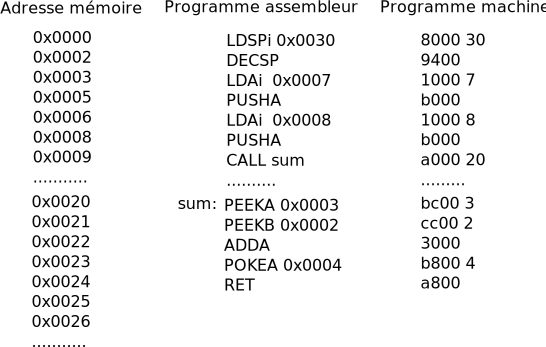
\includegraphics[width=0.7\linewidth]{Figs/traduction_asm_machine_call.pdf}

Assembleur : programme traduisant langage d'assemblage $\rightarrow$ code machine.\\
Abus : programme assembleur = programme en langage d'assemblage
\end{frame}

\begin{frame}
\frametitle{Quelques éléments de syntaxe de \underline{notre} assembleur}
\begin{itemize}
\item On utilise les mnémoniques LDAi, LDBi, STA, CALL, ...
\item les valeurs en hexadécimal sans préfixe 0x
\item ``;'' commentaire
\item étiquettes : pour les branchements, pour les variables; spécial @stack@
\item pseudo-instructions : e.g. 
\begin{itemize}
\item DSW : allocation de variables globales; par convention en début de programme!
\end{itemize}
\end{itemize}
Les variables et les étiquettes ne doivent pas être interprétables en hexadécimal
\end{frame}


\begin{frame}
\frametitle{Disposition du programme et des données en mémoire (\underline{chez nous})}

\centering\includegraphics[width=0.45\linewidth]{Figs/mem_layout.pdf}

\end{frame}


\begin{frame}[fragile]
\frametitle{Traduction de quelques structures de contrôle}

\begin{algorithmic}[1]
\While{$i \neq 0$}
\State{$res \gets res + i$}
\State{$i \gets i - 1$}
\EndWhile
\end{algorithmic}
\begin{small}
\begin{verbatim}
loop: LDAd i
      JZA  end
      LDBd res
      ADDB
      STB  res
      LDBi 1
      SUBA
      STA  i
      JMP  loop
end:  ...
\end{verbatim}
\end{small}
\end{frame}

\begin{frame}
\frametitle{Traduction de quelques structures de contrôle}
\begin{block}{for $\Leftrightarrow$ while}

\begin{small}
\begin{algorithmic}[1]
\For{$i = 0 ; i < N ; i = i + 1$}
\State{$res \gets res + i$}
\EndFor
\end{algorithmic}

\centering $\Leftrightarrow$

\begin{algorithmic}[1]
\State{$i \gets 0$}
\While{$i < N$}
\State{$res \gets res + i$}
\State{$i \gets i + 1$}
\EndWhile
\end{algorithmic}
\end{small}
\end{block}

\begin{block}{for $\Leftrightarrow$ while}
\begin{small}
\begin{algorithmic}[1]
\For{(init; condition ; incrément)}
\State{action}
\EndFor
\end{algorithmic}

\begin{algorithmic}[1]
\State{init}
\While{condition}
\State{action}
\State{incrément}
\EndWhile
\end{algorithmic}
\end{small}
\end{block}

\end{frame}

\begin{frame}[fragile]
\frametitle{Traduction de quelques structures de contrôle}

\begin{algorithmic}[1]
\If{$x != 0$}
\State{$x \gets 1$}
\EndIf
\State{$x \gets x + 1$}
\end{algorithmic}

\begin{small}
\begin{verbatim}
      LDAd x
      JZA  end
      LDAi 1
      STA  x
end:  LDBi 1
      ADDA
      STA  x
\end{verbatim}
\end{small}
\end{frame}

\begin{frame}[fragile]
\frametitle{Traduction de quelques structures de contrôle}

\begin{algorithmic}[1]
\If{$x == 10$}
\State{$x \gets 0$}
\Else
\State{$x \gets x + 1$}
\EndIf
\end{algorithmic}

\begin{small}
\begin{verbatim}
       LDAd x
       LDBi A
       SUBB
       JZB  if 
else:  LDBi 1
       ADDA
       STA  x
       JMP  end
if:    LDAi 0
       STA  x
end: ....
\end{verbatim}
\end{small}
\end{frame}

\begin{frame}
\frametitle{L'assembleur : traduction en code machine}
\textbf{Exercice :} Assembler le programme 

\begin{algorithmic}[1]
\State{$u \gets 127$}
\While{True}
\State{$u \gets next(u)$}
\State{print($u$)}
\EndWhile
\Function{$next$}{$u$}
\If{$u$ pair}
\Return{$u/2$}
\Else
\Return{$3 u + 1$}
\EndIf
\EndFunction
\end{algorithmic}

Compteur d'emplacement, table des symboles, variables globals; cf syr.asm\\
Démo : python assemble.py

\end{frame}


\section{Langages de haut niveau}

\begin{frame}
\centering\textbf{Langage de haut niveau (Python, C, C++, Scala, ..)}\\

\includegraphics[width=0.2\linewidth]{Figs/C_plus_plus.pdf}\hfill\includegraphics[width=0.4\linewidth]{Figs/Python.pdf}
\end{frame}

\begin{frame}
\frametitle{Mais pourquoi ?}

\begin{block}{Assembleur}
\begin{itemize}
\item spécifique à une architecture
\item encore dur à programmer (\texttt{LDAd b; LDBd c; ADDA; STA a})
\item peu de vérification syntaxique: on peut ajouter des choux et des carottes
\end{itemize}
\end{block}
\begin{block}{Langage de haut niveau}
\begin{itemize}
\item indépendant de l'architecture
\item langage plus intuitif, e.g. $a = b + c$, structures de contrôle, définition de fonctions
\item vérification syntaxique
\end{itemize}
\end{block}

%\textcolor{red}{TODO !!!!!!!}
%quelques éléments de langages de haut niveau
\end{frame}

\begin{frame}
\frametitle{Langage : Interprété ou compilé}
\begin{block}{Langage compilé}
Un programme (compilateur) convertit le code source en code machine qui peut \underline{ensuite} être exécuté\\
Ex : C++/g++\\
g++ -S main.cc\\
g++ -o main main.cc ; hexdump -C main\\
./main
\end{block}
\begin{block}{Langage interprété}
Un programme (interpréteur) interprète ``à la volée'' le code source\\
Ex : Python/ python\\
python main.py\\
$\Rightarrow$ Machine virtuelle python
\end{block}
\end{frame}

\begin{frame}
\frametitle{Brève Anatomie d'un compilateur}
\includegraphics[width=\linewidth]{Figs/compilation_frontend_backend.pdf}\\
\vfill
Référence : ``The dragon book'' Aho, Lam, Sethi, Ullman
\end{frame}

\begin{frame}
\frametitle{La phase d'analyse (frontend)}
\begin{block}{Analyse lexicale}
Ségmentation et identification des lexèmes\\
\centering\includegraphics[width=0.5\linewidth]{Figs/lexing.pdf}
\end{block}
\begin{block}{Analyse syntaxique}
Construction d'un arbre syntaxique à partir des lexèmes et d'une grammaire du langage.\\
\centering\includegraphics[width=0.6\linewidth]{Figs/erreur_syntaxe.pdf}
\end{block}
\end{frame}

\begin{frame}
\frametitle{La phase d'analyse (frontend)}

\centering\includegraphics[width=\linewidth]{Figs/syntactic_tree.pdf}

\end{frame}

\begin{frame}
\frametitle{Génération et optimisation d'une représentation intermédiaire}
\begin{block}{Représentation intermédiaire}
\begin{itemize}
\item indépendante du langage source (C, C++, ..) et de l'architecture (x86, ARM, CentraleSupelec)
\item facile à produire, facile à convertir en code machine
\item optimisable
\end{itemize}
Ex : register transfer language, gimple, generic, three adress code, single static assignment, control flow graph, ...
\end{block}
\vfill
Référence : ``The dragon book'' Aho, Lam, Sethi, Ullman
\end{frame}

\begin{frame}
\frametitle{Exemple de représentation intermédiaire : Three Adress code}
\begin{block}{Eléments de syntaxe}
\begin{itemize}
\item opérations binaires : \texttt{x := y op z}
\item opérations unaires : \texttt{x:= op y}
\item copies : \texttt{x := y}
\item sauts (in)conditionnels : \texttt{goto L}; \texttt{If x relop y goto L}
\item procédures : \texttt{param x1},.. \texttt{call p}, \texttt{return y}
\item ...
\end{itemize}
\end{block}
\end{frame}

\begin{frame}[fragile]
\frametitle{Exemple de représentation intermédiaire : Three Adress code}
\lstset { %
    language=C++,
    backgroundcolor=\color{black!5}, % set backgroundcolor
    basicstyle=\footnotesize,% basic font setting
}

\begin{small}
\begin{minipage}[c]{0.4\linewidth}
\begin{lstlisting}
int x = 3;
int y = 2 + 7 + x;
int z = 2*y;
if(x < y) {
  z = x/2 + y/3;
}
else {
  z = x * y + y;
}
\end{lstlisting}
\end{minipage}
\begin{minipage}[c]{0.5\linewidth}
\begin{verbatim}
     x = 3;
     _t1 = 2 + 7;
     y = _t1 + x;
     z = 2 * y;
     _t2 = x < y;
     IfZ _t2 Goto _L0;
     _t3 = x / 2;
     _t4 = y / 3;
     z = _t3 + _t4
     Goto _L1
_L0: _t5 = x * y;
     z = _t5 + z;
_L1:
\end{verbatim}
\end{minipage}
\end{small}

\end{frame}

\begin{frame}
\frametitle{Exemple de représentation intermédiaire : Control Flow Graph (CFG)}

\centering\includegraphics[width=0.7\columnwidth]{Figs/three_adresses.pdf}

\end{frame}

\begin{frame}
\frametitle{Optimisation d'un CFG}

\begin{block}{}
Application répétée de quelques règles de simplification
\begin{itemize}
\item supprimer des affectations inutiles
\item remplacer des constantes : int x = 3; int y = x + 2 $\Rightarrow$ int x = 3 ; int y = 3 + 2;
\item calculer des expressions constantes : int y = 3 + 2; $\Rightarrow$ int y = 5
\end{itemize}
jusqu'à ce que plus aucune des règles ne soit applicable
\end{block}
\end{frame}

\begin{frame}
\frametitle{Optimisation d'un CFG}

\centering\includegraphics[width=0.7\columnwidth]{Figs/three_adresses_optimisation.pdf}

\end{frame}

\begin{frame}
\frametitle{La phase de synthèse (backend)}
\begin{block}{Représentation intermédiaire $\Rightarrow$ Code machine}
\begin{itemize}
\item génération du code machine de chacun des blocs
\item disposition en mémoire des blocs
\item optimisations éventuelles
\end{itemize}
\end{block}

\centering\includegraphics[width=\columnwidth]{Figs/compilation_synthese.pdf}

\end{frame}

\begin{frame}
\frametitle{Et voila}


\includegraphics[width=\linewidth]{Figs/compilation_frontend_backend.pdf}\\
\vfill
Référence : ``The dragon book'' Aho, Lam, Sethi, Ullman

\end{frame}


%% \section{Procédures, pile et pointeur de pile}
%% \section{Traduction, compilation, interprétation}
%% \section{Les mémoires}
%% \section{Les périphériques}
%% \section{Les interruptions}
%% \section{Suppléments}

%------------------------------------------------

%----------------------------------------------------------------------------------------

\end{document} 
